\documentclass[12pt]{article}

\usepackage{amsmath, mathtools}
\usepackage{amsfonts}
\usepackage{amssymb}
\usepackage{graphicx}
\usepackage{colortbl}
\usepackage{xr}
\usepackage{hyperref}
\usepackage{longtable}
\usepackage{xfrac}
\usepackage{tabularx}
\usepackage{float}
\usepackage{siunitx}
\usepackage{booktabs}
\usepackage{caption}
\usepackage{pdflscape}
\usepackage{afterpage}

\usepackage[round]{natbib}

%\usepackage{refcheck}

\hypersetup{
    bookmarks=true,         % show bookmarks bar?
      colorlinks=true,       % false: boxed links; true: colored links
    linkcolor=red,          % color of internal links (change box color with linkbordercolor)
    citecolor=green,        % color of links to bibliography
    filecolor=magenta,      % color of file links
    urlcolor=cyan           % color of external links
}

%% Comments

\usepackage{color}

\newif\ifcomments\commentstrue

\ifcomments
\newcommand{\authornote}[3]{\textcolor{#1}{[#3 ---#2]}}
\newcommand{\todo}[1]{\textcolor{red}{[TODO: #1]}}
\else
\newcommand{\authornote}[3]{}
\newcommand{\todo}[1]{}
\fi

\newcommand{\wss}[1]{\authornote{blue}{SS}{#1}}
\newcommand{\an}[1]{\authornote{magenta}{Author}{#1}}
\newcommand{\wss}[1]{\authornote{blue}{SS}{#1}}



% For easy change of table widths
\newcommand{\colZwidth}{1.0\textwidth}
\newcommand{\colAwidth}{0.13\textwidth}
\newcommand{\colBwidth}{0.82\textwidth}
\newcommand{\colCwidth}{0.1\textwidth}
\newcommand{\colDwidth}{0.05\textwidth}
\newcommand{\colEwidth}{0.8\textwidth}
\newcommand{\colFwidth}{0.17\textwidth}
\newcommand{\colGwidth}{0.5\textwidth}
\newcommand{\colHwidth}{0.28\textwidth}

% Used so that cross-references have a meaningful prefix
\newcounter{defnum} %Definition Number
\newcommand{\dthedefnum}{GD\thedefnum}
\newcommand{\dref}[1]{GD\ref{#1}}
\newcounter{datadefnum} %Datadefinition Number
\newcommand{\ddthedatadefnum}{DD\thedatadefnum}
\newcommand{\ddref}[1]{DD\ref{#1}}
\newcounter{theorynum} %Theory Number
\newcommand{\tthetheorynum}{T\thetheorynum}
\newcommand{\tref}[1]{T\ref{#1}}
\newcounter{tablenum} %Table Number
\newcommand{\tbthetablenum}{T\thetablenum}
\newcommand{\tbref}[1]{TB\ref{#1}}
\newcounter{assumpnum} %Assumption Number
\newcommand{\atheassumpnum}{P\theassumpnum}
\newcommand{\aref}[1]{A\ref{#1}}
\newcounter{goalnum} %Goal Number
\newcommand{\gthegoalnum}{P\thegoalnum}
\newcommand{\gsref}[1]{GS\ref{#1}}
\newcounter{instnum} %Instance Number
\newcommand{\itheinstnum}{IM\theinstnum}
\newcommand{\iref}[1]{IM\ref{#1}}
\newcounter{reqnum} %Requirement Number
\newcommand{\rthereqnum}{P\thereqnum}
\newcommand{\rref}[1]{R\ref{#1}}
\newcounter{lcnum} %Likely change number
\newcommand{\lthelcnum}{LC\thelcnum}
\newcommand{\lcref}[1]{LC\ref{#1}}

\newcommand{\famname}{FFT} % PUT YOUR PROGRAM NAME HERE

\usepackage{fullpage}

\begin{document}

\title{FFT Library} 
\author{Yuzhi Zhao}
\date{\today}

\maketitle


\newpage

\tableofcontents

~\newpage

\pagenumbering{roman}

\section{Revision History}

\begin{tabularx}{\textwidth}{p{3cm}p{2cm}X}
\toprule {\bf Date} & {\bf Version} & {\bf Notes}\\
\midrule
Date 1 & 1.0 & Notes\\
Date 2 & 1.1 & Notes\\
\bottomrule
\end{tabularx}

~\newpage
	
\section{Reference Material}

This section records information for easy reference.

\subsection{Table of Units}

Throughout this document SI (Syst\`{e}me International d'Unit\'{e}s) is employed
as the unit system.  In addition to the basic units, several derived units are
used as described below.  For each unit, the symbol is given followed by a
description of the unit and the SI name.
~\newline

\renewcommand{\arraystretch}{1.2}
%\begin{table}[ht]
  \noindent \begin{tabular}{l l l} 
    \toprule		
    \textbf{symbol} & \textbf{unit} & \textbf{SI}\\
    \midrule 
    \si{\volt} & voltage & volt\\
    \si{\watt} & power & Watt (W = \si{\joule\per\second})\\
    \si{\hertz} &frequency& Hertz\\
    \si{\decibel} & decibel & Decibel\\
    \bottomrule
  \end{tabular}
  %	\caption{Provide a caption}
%\end{table}

\subsection{Table of Symbols}

The table that follows summarizes the symbols used in this document along with
their units.  The choice of symbols was made to be consistent with the heat
transfer literature and with existing documentation for solar water heating
systems.  The symbols are listed in alphabetical order.

\renewcommand{\arraystretch}{1.2}
%\noindent \begin{tabularx}{1.0\textwidth}{l l X}
\noindent \begin{longtable*}{l l p{12cm}} \toprule
\textbf{symbol} & \textbf{unit} & \textbf{description}\\
\midrule 
$A_C$ & \si[per-mode=symbol] {\square\metre} & coil surface area
\\
$A_\text{in}$ & \si[per-mode=symbol] {\square\metre} & surface area over 
which heat is transferred in
\\ 
\bottomrule
\end{longtable*}
\wss{Use your problems actual symbols.  The si package is a good idea to use for
  units.}

\subsection{Abbreviations and Acronyms}

\renewcommand{\arraystretch}{1.2}
\begin{tabular}{l l} 
  \toprule		
  \textbf{symbol} & \textbf{description}\\
  \midrule 
  A & Assumption\\
  DD & Data Definition\\
  GS & Goal Statement\\
  IM & Instance Model\\
  SRS & Software Requirements Specification\\
  \famname{} & Fast Fourier Transform\\
  T & Theoretical Model\\
  DFT & Discrete Fourier Transform\\
  IDFT & Invers Discrete Transform\\
  \bottomrule
\end{tabular}\\

\pagenumbering{arabic}

\section{Introduction}

\wss{This CA template is based on \citet{Smith2006}.  It
  will get you started, but you will have to make changes.  Any changes to
  section headings should be approved by the instructor, since that implies a
  deviation from the template.  Although the bits shown below do not include
  type information, you may need to add this information for your problem.}

\wss{Feel free to change the appearance of the report by modifying the LaTeX
  commands.}

\subsection{Purpose of Document}

This document will be  used as a starting point for subsequent development phases, including writing the design specification and the software verification and validation plan.
The design document will show how the requirements are to be realized, including decisions on the numerical algorithms and programming environment.
The verification and validation plan will show the steps that will be used to increase confidence in the software documentation and the implementation.


\subsection{Scope of the Family} 

The scope of the requirements includes specifing the input data, specifying the number of radix of FFT. Given the full information of input and parameters, the FFT Library will
take advantage of FFT algorithms to do DFT or IDFT calcualtion effectively.


\subsection{Characteristics of Intended Reader} 

Reviewers of this documentation should have a  strong knowledge in Complex Variables Functions as well as have an understanding of differential equaltions. 

\subsection{Organization of Document}
The organization of this document follows the template for an SRS for scientific
computing software proposed by~\cite{Koothoor2013} and \cite{SmithAndLai2005}.
The presentation follows the standard pattern of presenting goals, theories,
definitions, and assumptions.  For readers that would like a more bottom up
approach, they can start reading the instance models in Section
\ref{sec_instance} and trace back to find any additional information they
require.  The instance models provide the algebraic equations that model the FFT algorithm.


\section{General System Description}

This section identifies the interfaces between the system and its environment,
describes the potential user characteristics and lists the potential system
constraints.

\subsection{Potential System Contexts}
Figure~\ref{Fig_SystemContext} shows the system context.  A circle represents an
external entity outside the software, the user in this case.  A rectangle
represents the software system itself (\famname{}).  Arrows are used to show the data
flow between the system and its environment.\\


\begin{figure}[h!]
\begin{center}
 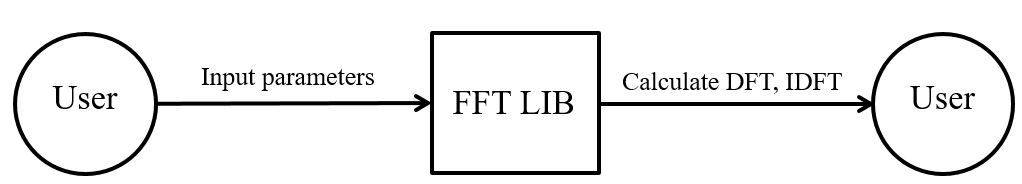
\includegraphics[width=0.6\textwidth]{SystemContextFigure}
\caption{System Context}
\label{Fig_SystemContext} 
\end{center}
\end{figure}

\begin{itemize}
\item User Responsibilities:
\begin{itemize}
\item  Provide the input data to the system, ensuring no errors in the data entry
\item  Make sure invoking the right functions according to different input data type
\end{itemize}
\item \famname{} Responsibilities:
\begin{itemize}
\item Determine if the inputs satisfy the required data type and format
\item Calculate the required outputs
\end{itemize}
\end{itemize}

\subsection{Potential User Characteristics} \label{SecUserCharacteristics}

The end user of \famname{} should have an understanding of undergraduate Level
1 Calculus and Physics.

\subsection{Potential System Constraints}
Not Applicable.

\section{Commonalities}

\subsection{Background Overview} \label{Sec_Background}


\subsection{Terminology and  Definitions}

This subsection provides a list of terms that are used in the subsequent
sections and their meaning, with the purpose of reducing ambiguity and making it
easier to correctly understand the requirements:

\begin{itemize}
\item Disceret Fourier Transform(DFT): A transform method to convert a signal from its original domain (often time or space) to a representation in the frequency domain.
\end{itemize}

\begin{itemize}
\item Inverse Disceret Fourier Transform(IDFT): A inverse transform method of DFT. 
\end{itemize}

\begin{itemize}
\item Fast Fourier Transform(FFT): A fast algorithm computes the discrete Fourier transform (DFT) of a sequence.
\end{itemize}

\begin{itemize}
\item Inverse Fast Fourier Transform(IFFT): A fast algorithm computes the inverse discrete Fourier transform (IDFT) of a sequence.
\end{itemize}

\subsection{Data Definitions} \label{sec_datadef}

This section collects and defines all the data needed to build the instance
models. The dimension of each quantity is also given.  
~\newline

\noindent
\begin{minipage}{\textwidth}
\renewcommand*{\arraystretch}{1.5}
\begin{tabular}{| p{\colAwidth} | p{\colBwidth}|}
\hline
\rowcolor[gray]{0.9}
Number& DD\refstepcounter{datadefnum}\thedatadefnum \label{FluxCoil}\\
\hline
Label& \bf A symbol represents ${e}^{-2\pi i/N}$ \\
\hline
Symbol & ${W}_N$\\
\hline
% Units& $Mt^{-3}$\\
% \hline
  SI Units & None\\
  \hline
  Equation& ${W}_N = {e}^{-2\pi i/N}$\\
  \hline
  Description & 
                ${W}_N$ is a simpler term to represent $ {e}^{-2\pi i/N} $. Readers can analyse complex-structure equations more directly and focus more on transformation process.
  \\
  \hline
  Sources& Commently Admitted \\
  \hline
  Ref.\ By & \iref{ewat}\\
  \hline
\end{tabular}
\end{minipage}\\


~\newline

\noindent
\begin{minipage}{\textwidth}
\renewcommand*{\arraystretch}{1.5}
\begin{tabular}{| p{\colAwidth} | p{\colBwidth}|}
\hline
\rowcolor[gray]{0.9}
Number& DD\refstepcounter{datadefnum}\thedatadefnum \label{FluxCoil}\\
\hline
Label& \bf Power Spectral Density (PSD)\\
\hline
Symbol & ${X}[k]$\\
\hline
% Units& $Mt^{-3}$\\
% \hline
  SI Units & \si{\watt\per\hertz}\\
  \hline
  Equation& ${X}[k] = {X}[0] + {X}[1] + {X}[2] + ..., (k = 0, 1, 2, 3...)$\\
  \hline
  Description & 
 Power spectral density (PSD) shows the strength of the variations(energy) as a function of frequency. In other words, it shows at which frequencies variations are strong and at which frequencies variations are weak.
  \\
  \hline
  Sources& \url{ http://www.cygres.com/OcnPageE/Glosry/SpecE.html }\\
  \hline
  Ref.\ By & \iref{ewat}\\
  \hline
\end{tabular}
\end{minipage}\\

~\newline

\noindent
\begin{minipage}{\textwidth}
\renewcommand*{\arraystretch}{1.5}
\begin{tabular}{| p{\colAwidth} | p{\colBwidth}|}
\hline
\rowcolor[gray]{0.9}
Number& DD\refstepcounter{datadefnum}\thedatadefnum \label{FluxCoil}\\
\hline
Label& \bf Amplitude Function\\
\hline
Symbol & ${x}(n)$\\
\hline
% Units& $Mt^{-3}$\\
% \hline
  SI Units & \si{\decibel}\\
  \hline
  Equation& Usually obtained from detector or other equipment directly.\\
  \hline
  Description & 
The amplitude of a periodic variable is a measure of its change over a single period (such as time or spatial period).  \\
  \hline
  Sources& \url{https://en.wikipedia.org/wiki/Amplitude }\\
  \hline
  Ref.\ By & \iref{ewat}\\
  \hline
\end{tabular}
\end{minipage}\\

~\newline

\noindent
\begin{minipage}{\textwidth}
\renewcommand*{\arraystretch}{1.5}
\begin{tabular}{| p{\colAwidth} | p{\colBwidth}|}
\hline
\rowcolor[gray]{0.9}
Number& DD\refstepcounter{datadefnum}\thedatadefnum \label{FluxCoil}\\
\hline
Label& \bf The Odd Terms OF Power Spectral Density\\
\hline
Symbol & ${X}[k]$\\
\hline
% Units& $Mt^{-3}$\\
% \hline
  SI Units & \si{\watt\per\hertz}\\
  \hline
  Equation& ${X}_E[k] = {X}[1] + {X}[3] + ..., (k = 1, 3, 5...)$\\
  \hline
  Description & 
The odd term set of the complete PSD but keeping the same physical meaning as PSD.
  \\
  \hline
  Sources& \\
  \hline
  Ref.\ By & \iref{ewat}\\
  \hline
\end{tabular}
\end{minipage}\\


~\newline

\noindent
\begin{minipage}{\textwidth}
\renewcommand*{\arraystretch}{1.5}
\begin{tabular}{| p{\colAwidth} | p{\colBwidth}|}
\hline
\rowcolor[gray]{0.9}
Number& DD\refstepcounter{datadefnum}\thedatadefnum \label{FluxCoil}\\
\hline
Label& \bf The Even Terms OF Power Spectral Density\\
\hline
Symbol & ${X}_O[k]$\\
\hline
% Units& $Mt^{-3}$\\
% \hline
  SI Units & \si{\watt\per\hertz}\\
  \hline
  Equation&  ${X}_O[k] = {X}[0] + {X}[2] + ..., (k = 0, 2, 4...)$\\
  \hline
  Description & 
The even term set of the complete PSD but keeping the same physical meaning as PSD.
  \\
  \hline
  Sources& \\
  \hline
  Ref.\ By & \iref{ewat}\\
  \hline
\end{tabular}
\end{minipage}\\





\subsection{Goal Statements}

\noindent Given the input data array of ${x}(n)$ or ${X}[k]$, radix r, the goal statements are:

\begin{itemize}

\item[GS\refstepcounter{goalnum}\thegoalnum \label{G_meaningfulLabel}:]Complete radix-2 FFT and IFFT when input is real data.
\item[GS\refstepcounter{goalnum}\thegoalnum \label{G_meaningfulLabel}:]Complete radix-2 FFT and IFFT when input is complex data.
\item[GS\refstepcounter{goalnum}\thegoalnum \label{G_meaningfulLabel}:]Complete radix-3 FFT and IFFT when input is real data.
\item[GS\refstepcounter{goalnum}\thegoalnum \label{G_meaningfulLabel}:]Complete radix-3 FFT  and IFFTwhen input is complex data.

\end{itemize}

\subsection{Theoretical Models} \label{sec_theoretical}

This section focuses on the general equations and laws that \famname{} is based
on. 

~\newline

\noindent
\begin{minipage}{\textwidth}
\renewcommand*{\arraystretch}{1.5}
\begin{tabular}{| p{\colAwidth} | p{\colBwidth}|}
  \hline
  \rowcolor[gray]{0.9}
  Number& T\refstepcounter{theorynum}\thetheorynum \label{T_DFT}\\
  \hline
  Label&\bf Discrete Fourier Transform(DFT)\\
  \hline
  Equation & ${X}[k]$ = $\sum\limits_{n=0}^{N-1} x(n)$ $ {e}^{-2\pi ni/N} $ \\
  \hline
  Description & 
                The above equation is the defination of Discrete Fourier Transform, which transforms a sequence of N complex numbers ${x}(0)$,  ${x}(1)$,  ${x}(2)$,  ${x}(3)$... into another sequence of complex numbers,  ${X}[0]$,  ${X}[1]$,  ${X}[2]$,  ${X}[3]$,  ${X}[4]$...In the equation, ${x}(n)$ is amplitude in time domain and  ${e}^{-2\pi i/N}$  is an important term in DFT algorithm.\\
  \hline
  Source &
           \url  {https://en.wikipedia.org/wiki/Discrete_Fourier_transform}\\
  % The above web link should be replaced with a proper citation to a publication
  \hline
  Ref.\ By & \dref{ROCT}\\
  \hline
\end{tabular}
\end{minipage}\\

~\newline

\noindent
\begin{minipage}{\textwidth}
\renewcommand*{\arraystretch}{1.5}
\begin{tabular}{| p{\colAwidth} | p{\colBwidth}|}
  \hline
  \rowcolor[gray]{0.9}
  Number& T\refstepcounter{theorynum}\thetheorynum \label{T_IDFT}\\
  \hline
  Label&\bf Inverse Discrete Fourier Transform(IDFT)\\
  \hline
  Equation&  ${x}(n)$ = $\frac{1}{N}$ $\sum\limits_{n=0}^{N-1} X[k]$ $ {e}^{2\pi ni/N} $\\
  \hline
  Description & 
                The above equation is the defination of Inverse Discrete Fourier Transform, which transforms a sequence of N complex numbers ${X}[0]$,  ${X}[1]$,  ${X}[2]$,  ${X}[3]$,  ${X}[4]$... into another sequence of complex numbers, ${x}(0)$,  ${x}(1)$,  ${x}(2)$,  ${x}(3)$...In the equation, ${X}[k]$ is amplitude in time domain and  ${e}^{-2\pi i/N}$  is an important term in IDFT algorithm, while N is the length of sequence.\\
  \hline
  Source &
          \url  {https://en.wikipedia.org/wiki/Discrete_Fourier_transform}\\
  % The above web link should be replaced with a proper citation to a publication
  \hline
  Ref.\ By & \dref{ROCT}\\
  \hline
\end{tabular}
\end{minipage}\\


~\newline

\noindent
\begin{minipage}{\textwidth}
\renewcommand*{\arraystretch}{1.5}
\begin{tabular}{| p{\colAwidth} | p{\colBwidth}|}
  \hline
  \rowcolor[gray]{0.9}
  Number& T\refstepcounter{theorynum}\thetheorynum \label{T_EF}\\
  \hline
  Label&\bf Euler's Formula\\
  \hline
  Equation& ${e}^{ix}$ = $cosx$ + $isinx$\\
  \hline
  Description & 
Euler's formula, named after Leonhard Euler, is a mathematical formula in complex analysis that establishes the fundamental relationship between the trigonometric functions and the complex exponential function. ${e}$ is the base of the natural logarithm, i is the imaginary unit, and cos and sin are the trigonometric functions cosine and sine respectively, with the argument x given in radians. \\
  \hline
  Source &
          \url {https://en.wikipedia.org/wiki/Euler%27s_formula} \\
  % The above web link should be replaced with a proper citation to a publication
  \hline
  Ref.\ By & \dref{ROCT}\\
  \hline
\end{tabular}
\end{minipage}\\

~\newline

\noindent
\begin{minipage}{\textwidth}
\renewcommand*{\arraystretch}{1.5}
\begin{tabular}{| p{\colAwidth} | p{\colBwidth}|}
  \hline
  \rowcolor[gray]{0.9}
  Number& T\refstepcounter{theorynum}\thetheorynum \label{T_POW}\\
  \hline
  Label&\bf Periodicity Of $W_N^{kn}$\\
  \hline
  Equation& $W_N^{kn}$ =  $W_N^{k(n+N)}$\\
  \hline
  Description & 
 $W_N^{kn}$ is a periodic function and the period is N. Using Euler's Formula can prove this.
\\
  \hline
  Source &
          \url {https://en.wikipedia.org/wiki/Euler%27s_formula} \\
  % The above web link should be replaced with a proper citation to a publication
  \hline
  Ref.\ By & \dref{ROCT}\\
  \hline
\end{tabular}
\end{minipage}\\

~\newline

\noindent
\begin{minipage}{\textwidth}
\renewcommand*{\arraystretch}{1.5}
\begin{tabular}{| p{\colAwidth} | p{\colBwidth}|}
  \hline
  \rowcolor[gray]{0.9}
  Number& T\refstepcounter{theorynum}\thetheorynum \label{T_TOWS}\\
  \hline
  Label&\bf A Transform Of $W_N^{kn}$\\
  \hline
  Equation& $W_N^{akn}$ =  $W_{N/a}^{kn}$\\
  \hline
  Description & 
a is a coefficient. This transform is frequently used in FFT algorithms.
\\
  \hline
  Source & \\
  % The above web link should be replaced with a proper citation to a publication
  \hline
  Ref.\ By & \dref{ROCT}\\
  \hline
\end{tabular}
\end{minipage}\\

~\newline

\subsection{Instance Models} \label{sec_instance}

~\newline

%Instance Model 1

\noindent
\begin{minipage}{\textwidth}
\renewcommand*{\arraystretch}{1.5}
\begin{tabular}{| p{\colAwidth} | p{\colBwidth}|}
  \hline
  \rowcolor[gray]{0.9}
  Number& IM\refstepcounter{instnum}\theinstnum \label{ewat}\\
  \hline
  Label& \bf Radix-2 FFT Calculation\\
  \hline
  Input& $a_n$, $b_n$, N, r from \iref{epcm}\\
  &The input is constrained so that $N \leq 20$, r = 2.\\
  \hline
  Output& X[k], k =(0, 1, ...,  N),  in format 'a + bi'\\
  \hline
  Description& X[k] is the power spectral density (\si{\watt\per\hertz}),\\
&a is the real number part,\\
&b is the coefficient part of complex number part.\\
  \hline
  Sources&~\cite{Lightstone2012} \ \\
  \hline
  Ref.\ By & \iref{epcm}\\
  \hline
\end{tabular}
\end{minipage}\\

\subsubsection*{Detailed Radix-2 FFT Algirithm}

\begin{align*}
X[k] &= \sum\limits_{n=0}^{N-1}x(n)W_{N}^{kn}\\
& = \sum\limits_{even}x(n)W_{N}^{kn} + \sum\limits_{odd}x(n)W_{N}^{kn}\\
\end{align*}

Define n = 2r and n = 2r + 1, r = 0, 1, 2, ..., N/2 -1.\\

\begin{align*}
X[k] &= \sum\limits_{r=0}^{N/2 -1}x(2r)W_{N}^{2kr} + \sum\limits_{r=0}^{N/2 -1}x(2r+1)W_{N}^{(2r+ 1)k}\\
& =  \sum\limits_{r=0}^{N/2 -1}x(2r)(W_{N}^{2})^{kr} + W_{N}^{k}\sum\limits_{r=0}^{N/2 -1}x(2r+1)(W_{N}^{2})^{kr}\\
\end{align*}

According to Eular's Formula, $W_{N}^{a}$ = $W_{N/a}$,\\

\begin{align*}
X[k] & =  \sum\limits_{r=0}^{N/2 -1}x(2r)(W_{N}^{2})^{kr} + W_{N}^{k}\sum\limits_{r=0}^{N/2 -1}x(2r+1)(W_{N}^{2})^{kr}\\
& = \sum\limits_{r=0}^{N/2 -1}x(2r)(W_{N/2})^{kr} + W_{N}^{k}\sum\limits_{r=0}^{N/2 -1}x(2r+1)(W_{N/2})^{kr}\\
& = X_e[k] + W_N^kX_o[k]\\S
\end{align*}

We can use FFT butterfly diagram to analysis a  FFT computing process and we can clearly tell how the sequence is divided and computed. Here we will have a simplest
N = 8, radix-2, butterfly diagram as example:\\

Figure~\ref{Fig_Radix-2FFT}

\begin{figure}[h!]
\begin{center}
 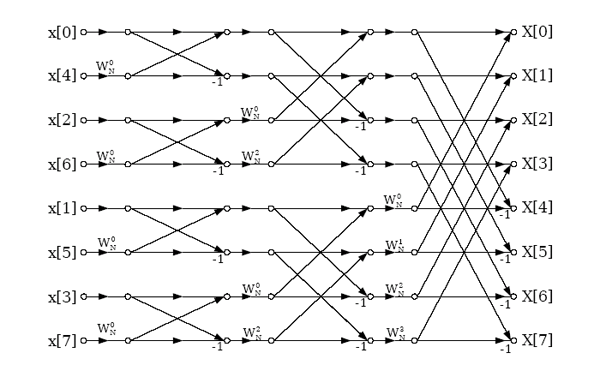
\includegraphics[width=0.6\textwidth]{butterflyRedix2}
\caption{Radix-2 8-Point FFT}
\label{Fig_Radix-2FFT}
\end{center}
\end{figure}

From the diagram, there were twice times of division of even and odd sequences. The first time division spilt the even and odd sequences. The second time, we took even and odd sequences retrieved from last division as two new sequences and split both of them into the even and odd sequences again. So far from the lowest level, we can consider our original sequence as a four-piece sequences. And then we can compute the sequence from the lowest level. Thus, we can develop our algorithm to a bigger domain. Unless the number of terms
in a sequence is in pattern of  $2^s$($s\in\mathbb{Z}$, s $<$ 20), the sequence can be reduced until the smallest piece is consist of two terms.\\
\\
Radix-2 IFFT implements the same algorithim.\\

~\newline

%Instance Model 2

\noindent
\begin{minipage}{\textwidth}
\renewcommand*{\arraystretch}{1.5}
\begin{tabular}{| p{\colAwidth} | p{\colBwidth}|}
  \hline
  \rowcolor[gray]{0.9}
  Number& IM\refstepcounter{instnum}\theinstnum \label{ewat}\\
  \hline
  Label& \bf Radix-3 FFT Calculation\\
  \hline
  Input& $a_n$, $b_n$, N, r from \iref{epcm}\\
  &The input is constrained so that $N \leq 20$, r = 3.\\
  \hline
  Output& X[k], k =(0, 1, ...,  N),  in format 'a + bi'\\
  \hline
  Description& X[k] is the power spectral density (\si{\watt\per\hertz}),\\
&a is the real number part,\\
&b is the coefficient part of complex number part.\\
  \hline
  Sources&~\cite{Lightstone2012} \ \\
  \hline
  Ref.\ By & \iref{epcm}\\
  \hline
\end{tabular}
\end{minipage}\\

\subsubsection*{Detailed Radix-3 FFT Algirithm}

\begin{align*}
X[k] &= \sum\limits_{n=0}^{N-1}x(n)W_{N}^{kn}\\
& = \sum\limits_{n = 3^r}x(n)W_{N}^{kn} + \sum\limits_{n = 3^r+1}x(n)W_{N}^{kn} + \sum\limits_{n = 3^r+2}x(n)W_{N}^{kn}\\
& = \sum\limits x_1(n)W_{N}^{kn} + \sum\limits x_2(n)W_{N}^{kn} + \sum\limits x_3(n)W_{N}^{kn}  ()\\
\end{align*}


Define n = 3r, n = 3r + 1 and n = 3r +2, r = 0, 1, 2, ..., N/3 -1.\\

\begin{align*}
X[k] &= \sum\limits_{r=0}^{N/3 -1}x(3r)W_{N}^{3kr} + \sum\limits_{r=0}^{N/3 -1}x(3r+1)W_{N}^{(3r+ 1)k} + \sum\limits_{r=0}^{N/3 -1}x(3r+2)W_{N}^{(3r+ 2)k}\\
& =  \sum\limits_{r=0}^{N/3 -1}x(3r)(W_{N}^{3})^{kr} + W_{N}^{k}\sum\limits_{r=0}^{N/3 -1}x(3r+1)(W_{N}^{3})^{kr} + W_{N}^{2k}\sum\limits_{r=0}^{N/3 -1}x(3r+2)(W_{N}^{3})^{kr}\\
\end{align*}

According to Eular's Formula, $W_{N}^{a}$ = $W_{N/a}$,\\

\begin{align*}
X[k] & =  \sum\limits_{r=0}^{N/3 -1}x(3r)(W_{N}^{3})^{kr} + W_{N}^{k}\sum\limits_{r=0}^{N/3 -1}x(3r+1)(W_{N}^{3})^{kr} + W_{N}^{2k}\sum\limits_{r=0}^{N/3 -1}x(3r+2)(W_{N}^{3})^{kr}\\
& = \sum\limits_{r=0}^{N/3 -1}x(3r)(W_{N/3})^{kr} + W_{N}^{k}\sum\limits_{r=0}^{N/3 -1}x(3r+1)(W_{N/3})^{kr} + W_{N}^{2k}\sum\limits_{r=0}^{N/3 -1}x(3r+2)(W_{N/3})^{kr}\\
& = X_1[k] + W_N^kX_2[k] + W_N^{2k}X_3[k]\\
\end{align*}

We can use FFT butterfly diagram to analysis a FFT computing process and we can clearly tell how the sequence is divided and computed. Here we will have a simplest
N = 9, radix-3, butterfly diagram as example:\\
\\
\\
Figure~\ref{Fig_Radix-3FFT}

\begin{figure}[h!]
\begin{center}
 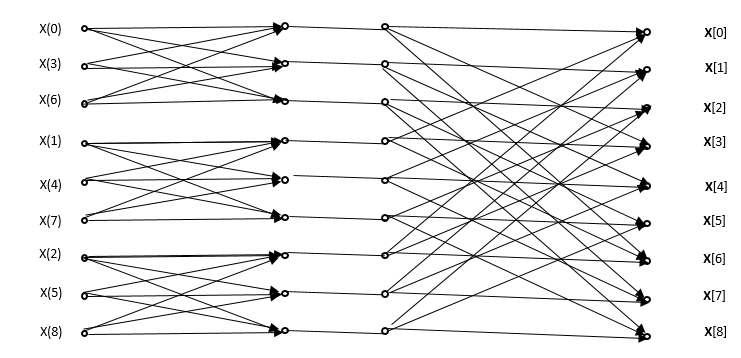
\includegraphics[width=0.6\textwidth]{butterflyRedix3}
\caption{Radix-3 9-Point FFT}
\label{Fig_Radix-3FFT}
\end{center}
\end{figure}

From the diagram, there were two times of division of sequences. Each division split sequence into three parts. The first sequence is the sum of all terms whose sequence number can be divided by 3 without the rest. The second sequence is the sum of all terms whose sequence number can be divided by 3 with rest of 1. The third sequence is the sum of all terms whose sequence number can be divided by 3 with the rest of 2. The first time division spilt the sequence into three parts following the rules as mentioned. The second time, we implement the same rule to split these three sequences so that each sequence is divided into three sequences. So far from the lowest level, we can consider our original sequence as a nine-piece sequences. And then we can compute the sequence from the lowest level. Thus, we can develop our algorithm to a bigger domain. Unless the number of terms
in a sequence is in pattern of  $3^s$($s\in\mathbb{Z}$, s $<$ 20), the sequence can be reduced until the smallest piece is consist of three terms.\\
\\
Radix-3 IFFT implements the same algorithim.\\



\section{Variabilities}

\subsection{Assumptions}

\begin{itemize}

\item[A\refstepcounter{assumpnum}\theassumpnum \label{A_meaningfulLabel}:]
The number of  input of radix-2 FFT and IFFT shoud be $2^s$($s\in\mathbb{Z}$, s $<$ 20) [\tref{T_DFT}].
\item[A\refstepcounter{assumpnum}\theassumpnum \label{A_meaningfulLabel}:]
The number of input of radix-3 FFT and IFFT should be $3^s$($s\in\mathbb{Z}$, s $<$ 20) [\tref{T_DFT}].
\item[A\refstepcounter{assumpnum}\theassumpnum \label{A_meaningfulLabel}:]
The length of $X[k] $sequence is always equal to the length of sequence $x(n)$  [\tref{T_DFT}].
\item[A\refstepcounter{assumpnum}\theassumpnum \label{A_meaningfulLabel}:]
The coefficient of every term in $x(n)$ is an integer for both complex and real number  [\tref{T_DFT}].
\item[A\refstepcounter{assumpnum}\theassumpnum \label{A_meaningfulLabel}:]
When retrieving the complex number FFT function, some terms are still real numbers. Users enter 0 as an coefficient for complex terms under this occation [\tref{T_DFT}].
\item[A\refstepcounter{assumpnum}\theassumpnum \label{A_meaningfulLabel}:]
Assume the strides for ${X}[n]$ and ${x}(n)$ are both 1.
\item[A\refstepcounter{assumpnum}\theassumpnum \label{A_meaningfulLabel}:]
The length of input sequence is known [\tref{T_DFT}].


\end{itemize}

\subsection{Calculation} \label{sec_Calculation}
Not Applicable.
\subsection{Output} \label{sec_Output}    
Not Applicable.



\section{Traceability Matrices and Graphs}
The purpose of the traceability matrices is to provide easy references on what has to be additionally modified if a certain component is changed.  Every time a 
component is changed, the items in the column of that component that are 
marked with an ``X'' should be modified as well.  Table~\ref{Table:trace}
shows the dependencies of theoretical models, general definitions, data
definitions, and instance models with each other. Table~\ref{Table:R_trace} shows
the dependencies of instance models, requirements, and data constraints on each other. Table~\ref{Table:A_trace} shows the dependencies of theoretical models, general definitions, data definitions,  instance models, and likely changes on the assumptions.

\afterpage{
\begin{landscape}
\begin{table}[h!]
\centering
\begin{tabular}{|c|c|c|c|c|c|c|c|c|c|c|c|c|c|c|c|c|c|c|c|}
\hline
	& \aref{A_OnlyThermalEnergy}& \aref{A_hcoeff}& \aref{A_mixed}& \aref{A_tpcm}& \aref{A_const_density}& \aref{A_const_C}& \aref{A_Newt_coil}& \aref{A_tcoil}& \aref{A_tlcoil}& \aref{A_Newt_pcm}& \aref{A_charge}& \aref{A_InitTemp}& \aref{A_OpRangePCM}& \aref{A_OpRange}& \aref{A_htank}& \aref{A_int_heat}& \aref{A_vpcm}& \aref{A_PCM_state}& \aref{A_Pressure} \\
\hline
\tref{T_DFT}        & X& & & & & & & & & & & & & & & & & & \\ \hline
\tref{T_IDFT}        & & & & & & & & & & & & & & & & & & & \\ \hline
\tref{T_EF}        & & & & & & & & & & & & & & & & & & & \\ \hline
\tref{T_POW}        & & & & & & & & & & & & & & & & & & & \\ \hline
\tref{T_TOW}        & & & & & & & & & & & & & & & & & & & \\ \hline
\dref{NL}           & & X& & & & & & & & & & & & & & & & & \\ \hline
\dref{ROCT}         & & & X& X& X& X& & & & & & & & & & & & & \\ \hline
\ddref{FluxCoil}    & & & & & & & X& X& X& & & & & & & & & & \\ \hline
\ddref{FluxPCM}     & & & X& X& & & & & & X& & & & & & & & & \\ \hline
\ddref{D_HOF}       & & & & & & & & & & & & & & & & & & & \\ \hline
\ddref{D_MF}        & & & & & & & & & & & & & & & & & & & \\ \hline
\iref{ewat}         & & & & & & & & & & & X& X& & X& X& X& & & X \\ \hline
\iref{epcm}         & & & & & & & & & & & & X& X& & & X& X& X& \\ \hline
\iref{I_HWAT}       & & & & & & & & & & & & & & X& & & & & X \\ \hline
\iref{I_HPCM}       & & & & & & & & & & & & & X& & & & & X & \\ \hline
\lcref{LC_tpcm}     & & & & X& & & & & & & & & & & & & & & \\ \hline
\lcref{LC_tcoil}    & & & & & & & & X& & & & & & & & & & & \\ \hline
\lcref{LC_tlcoil}   & & & & & & & & & X& & & & & & & & & & \\ \hline
\lcref{LC_charge}   & & & & & & & & & & & X& & & & & & & & \\ \hline
\lcref{LC_InitTemp} & & & & & & & & & & & & X& & & & & & & \\ \hline
\lcref{LC_htank}    & & & & & & & & & & & & & & & X& & & & \\
\hline
\end{tabular}
\caption{Traceability Matrix Showing the Connections Between Assumptions and Other Items}
\label{Table:A_trace}
\end{table}
\end{landscape}
}

\begin{table}[h!]
\centering
\begin{tabular}{|c|c|c|c|c|c|c|c|c|c|c|c|c|c|c|c|c|c|c|c|c|c|c|c|}
\hline        
	& \tref{T_DFT}& \tref{T_IDFT}& \tref{T_EF}& \tref{T_POW}& \tref{T_TOW}& \dref{NL}& \dref{ROCT} & \ddref{FluxCoil}& \ddref{FluxPCM} & \ddref{D_HOF}& \ddref{D_MF}& \iref{ewat}& \iref{epcm}& \iref{I_HWAT}& \iref{I_HPCM} \\
\hline
\tref{T_DFT}     & & & & & & & & & & & & & \\ \hline
\tref{T_IDFT}     & & & X& & & & & & & & & & \\ \hline
\tref{T_EF}     & & & & & & & & & & & & & \\ \hline
\tref{T_POW}     & & & X& & & & & & & & & & \\ \hline
\tref{T_TOW}     & & & & & & & & & & & & & \\ \hline
\dref{NL}        & & & & & & & & & & & & & \\ \hline
\dref{ROCT}      & X& & & & & & & & & & & & \\ \hline
\ddref{FluxCoil} & & & & X& & & & & & & & & \\ \hline
\ddref{FluxPCM}  & & & & X& & & & & & & & & \\ \hline
\ddref{D_HOF}    & & & & & & & & & & & & & \\ \hline
\ddref{D_MF}     & & & & & & & & X& & & & & \\ \hline
\iref{ewat}      & & & & & X& X& X& & & & X& & \\ \hline
\iref{epcm}      & & & & & X& & X& & X& X& & & X \\ \hline
\iref{I_HWAT}    & & X& & & & & & & & & & & \\ \hline
\iref{I_HPCM}    & & X& X& & & & X& X& X& & X& & \\
\hline
\end{tabular}
\caption{Traceability Matrix Showing the Connections Between Items of Different Sections}
\label{Table:trace}
\end{table}

\begin{table}[h!]
\centering
\begin{tabular}{|c|c|c|c|c|c|c|c|}
\hline
	& \iref{ewat}& \iref{epcm}& \iref{I_HWAT}& \iref{I_HPCM}& \ref{sec_DataConstraints}& \rref{R_RawInputs}& \rref{R_MassInputs} \\
\hline
\iref{ewat}            & & X& & & & X& X \\ \hline
\iref{epcm}            & X& & & X& & X& X \\ \hline
\iref{I_HWAT}          & & & & & & X& X \\ \hline
\iref{I_HPCM}          & & X& & & & X& X \\ \hline
\rref{R_RawInputs}     & & & & & & & \\ \hline
\rref{R_MassInputs}    & & & & & & X& \\ \hline
\rref{R_CheckInputs}   & & & & & X& & \\ \hline
\rref{R_OutputInputs}  & X& X& & & & X& X \\ \hline
\rref{R_TempWater}     & X& & & & & & \\ \hline 
\rref{R_TempPCM}       & & X& & & & & \\ \hline
\rref{R_EnergyWater}   & & & X& & & & \\ \hline
\rref{R_EnergyPCM}     & & & & X& & & \\ \hline
\rref{R_VerifyOutput}  & & & X& X& & & \\ \hline
\rref{R_timeMeltBegin} & & X& & & & & \\ \hline
\rref{R_timeMeltEnd}   & & X& & & & & \\ 
\hline
\end{tabular}
\caption{Traceability Matrix Showing the Connections Between Requirements and Instance Models}
\label{Table:R_trace}
\end{table}

The purpose of the traceability graphs is also to provide easy references on what has to be additionally modified if a certain component is changed.  The arrows in the graphs represent dependencies. The component at the tail of an arrow is depended on by the component at the head of that arrow. Therefore, if a component is changed, the components that it points to should also be changed. Figure~\ref{Fig_ATrace} shows the dependencies of theoretical models, general definitions, data definitions, 
instance models, likely changes, and assumptions on each other. Figure~\ref{Fig_RTrace} shows the dependencies of instance models, requirements, and data constraints on each other.\par
NOTE: Building a tool to automatically generate the graphical 
representation of the matrix by scanning the labels and reference can be 
future work.

\begin{figure}[h!]
	\begin{center}
		%\rotatebox{-90}
		{
			\includegraphics[width=\textwidth]{ATrace.png}
		}
		\caption{\label{Fig_ATrace} Traceability Matrix Showing the Connections Between Items of Different Sections}
	\end{center}
\end{figure}


\begin{figure}[h!]
	\begin{center}
		%\rotatebox{-90}
		{
			\includegraphics[width=0.7\textwidth]{RTrace.png}
		}
		\caption{\label{Fig_RTrace} Traceability Matrix Showing the Connections Between Requirements, Instance Models, and Data Constraints}
	\end{center}
\end{figure}


\wss{You will have to add tables.}

\newpage

\bibliographystyle {plainnat}
\bibliography {../../ReferenceMaterial/References}

\newpage

\section{Appendix}

\wss{Your report may require an appendix.  For instance, this is a good point to
show the values of the symbolic parameters introduced in the report.}

\subsection{Symbolic Parameters}

\wss{The definition of the requirements will likely call for SYMBOLIC\_CONSTANTS.
Their values are defined in this section for easy maintenance.}

\end{document}